\documentclass[../../main.tex]{subfiles}
\begin{document}

{\bf [解]}
まずは$f(x)$を求めよう．
被積分関数の絶対値の中身を
\begin{align}
 g(t,x)=\cos t-x\sin2t
\end{align}
とおくと，$\sin 2t=2\sin t\cos t$だから
\begin{align}
 g(t,x) 
  &= \cos t - 2x\sin t \cos t \\
  &= \cos t \left(1-2x\sin t\right) \label{eq:1}
\end{align}
である．
$0\le t\le\dfrac{\pi}{2}$で$\cos t\ge0,\sin t\ge 0$だからこの符号は$x \le 0$の時自明に正であり，$x > 0$の時は以下のようになる．
\begin{enumerate}
 \item[$x\le\dfrac{1}{2}$の時] $0\le t\le \dfrac{\pi}{2}$で$\sin t\le1\le\dfrac{1}{2x}$より$1-2x\sin t\ge0$，よって$g(t)\ge0$となる． \\
 \item[$x>\dfrac{1}{2}$の時] $0<t<\pi/2$に$\sin t=\dfrac{1}{2x}\in(0,1)$となる$t=\alpha$がただ1つ存在し，$0\le t\le\alpha$で$g(t)\ge0$，$\alpha\le t\le\pi/2$で$g(t)\le0$となる．
\end{enumerate}
以上より，$f(x)$の被積分関数の絶対値を外すと
\begin{align}
 f(x)&=
   \begin{cases}
       \displaystyle\int_0^{\pi/2}g(t)\,dt & \Bigl(x\le\dfrac{1}{2}\Bigr)\\[2mm]
       \displaystyle\int_0^\alpha g(t)\,dt-\int_\alpha^{\pi/2}g(t)\,dt & \Bigl(\dfrac{1}{2}\le x\Bigr)
   \end{cases} \label{eq:2}
\end{align}
となる．
$g(t)$の原始関数の1つとして
\begin{align}
 G(t)=\sin t+\dfrac{1}{2}x\cos2t
\end{align}
があるから，これを用いて
\begin{align}
 f(x)&=
   \begin{cases}
       \displaystyle G\left(\dfrac{\pi}{2}\right) - G(0)  & \Bigl(x\le\dfrac{1}{2}\Bigr)\\[2mm]
       \displaystyle 2G(\alpha) - G(0) - G\left(\dfrac{\pi}{2}\right)  & \Bigl(\dfrac{1}{2}\le x\Bigr)
   \end{cases} \label{eq:3}
\end{align}
である．各項計算すると
\begin{align}
 G(0) &= \dfrac{x}{2}\\
 G\left(\dfrac{\pi}{2}\right) &= 1 - \dfrac{x}{2} \\
 G(\alpha) &= 2\sin\alpha + x\cos 2\alpha \\
           &= 2\sin\alpha + x\left(1-\dfrac{\sin^2\alpha}{2}\right) \\
           &= \dfrac{1}{x} + x\left(1-\dfrac{1}{2x^2}\right)\quad (\because g(\alpha)=0) \\
           &= x + \dfrac{1}{2x}
\end{align}
だから\cref{eq:3}に代入して
\begin{align}
 f(x)&=
   \begin{cases}
       \displaystyle 1 - \dfrac{x}{2} - \dfrac{x}{2}  & \Bigl(x\le\dfrac{1}{2}\Bigr)\\[2mm]
       \displaystyle 2\left(x + \dfrac{1}{2x}\right) - \dfrac{x}{2} - \left(1 - \dfrac{x}{2}\right) & \Bigl(\dfrac{1}{2}\le x\Bigr)
   \end{cases} \\
&=
   \begin{cases}
       \displaystyle 1 - x  & \Bigl(x\le\dfrac{1}{2}\Bigr)\\[2mm]
       \displaystyle 2x  + \dfrac{1}{x} - 1 & \Bigl(\dfrac{1}{2}\le x\Bigr)
   \end{cases} \label{eq:4}
\end{align}
である．これを図示すると下図のようになる．

\begin{figure}[htb]
\centering
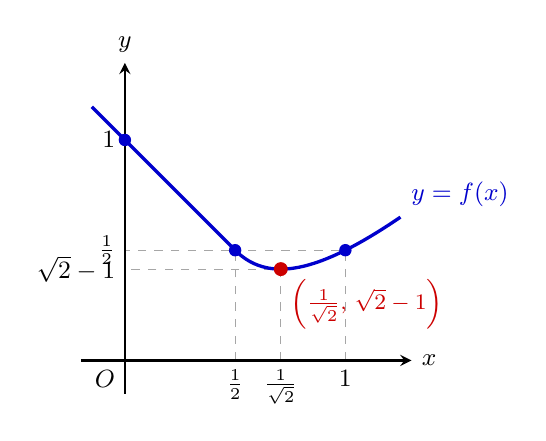
\begin{tikzpicture}[scale=2.8, >=stealth, every node/.style={font=\small}]

  % --- パラメータ定義 ---
  % x = 1/2 = 0.5, y(1/2) = 0.5
  % 最小点: x = 1/sqrt(2) \approx 0.7071, y = sqrt(2) - 1 \approx 0.4142
  % 端点: x = 1, y(1) = 0.5
  \def\xmin{-0.2}
  \def\xmax{1.3}

  % 1. 補助線（点線）
  % x = 1/2, y = 1/2
  \draw[dashed, gray!70] (0.5, 0) -- (0.5, 0.5) -- (0, 0.5);
  % 最小点 x = 1/\sqrt{2}, y = \sqrt{2} - 1
  \draw[dashed, gray!70] (0.7071, 0) -- (0.7071, 0.4142) -- (0, 0.4142);
  % x = 1, y = 1/2
  \draw[dashed, gray!70] (1.0, 0) -- (1.0, 0.5) -- (0.5, 0.5);

  % 2. 座標軸
  \draw[->, thick] (\xmin, 0) -- (\xmax, 0) node[right] {$x$};
  \draw[->, thick] (0, -0.15) -- (0, 1.35) node[above] {$y$};
  \node[below left] at (0,0) {$O$};

  % 3. グラフ描画
  % (i) x <= 1/2 の直線: y = 1 - x
  \draw[very thick, blue!80!black, domain=-0.15:0.5] 
    plot (\x, {1.0 - \x});

  % (ii) x >= 1/2 の曲線: y = x + 1/(2x) - 1
  \draw[very thick, blue!80!black, domain=0.5:1.25, smooth, samples=60] 
    plot (\x, {\x + 1.0/(2.0*\x) - 1.0}) node[above right] {$y = f(x)$};

  % 4. 軸上の目盛りテキスト
  \node[below] at (0.5, 0) {$\frac{1}{2}$};
  \node[below] at (0.7071, 0) {$\frac{1}{\sqrt{2}}$};
  \node[below] at (1.0, 0) {$1$};

  \node[left] at (0, 1.0) {$1$};
  \node[left] at (0, 0.5) {$\frac{1}{2}$};
  \node[left] at (0, 0.4142) {$\sqrt{2}-1$};

  % 5. 特徴的なプロット点
  % y切片 (0, 1)
  \fill[blue!80!black] (0, 1.0) circle (0.8pt);
  % 接続点 (1/2, 1/2)
  \fill[blue!80!black] (0.5, 0.5) circle (0.8pt);
  % 最小点 (1/\sqrt{2}, \sqrt{2}-1)
  \fill[red!80!black] (0.7071, 0.4142) circle (0.9pt) 
    node[below right, font=\footnotesize] {$\left(\frac{1}{\sqrt{2}},\,\sqrt{2}-1\right)$};
  % 点 (1, 1/2)
  \fill[blue!80!black] (1.0, 0.5) circle (0.8pt);

\end{tikzpicture}
\caption{関数 $y = f(x)$ のグラフ}
\end{figure}

\paragraph{(1)}

\cref{eq:4}より$x\le1/2$では$f(x)=1-x$は単調減少で最小値は
\begin{align}
 f\left(\dfrac{1}{2}\right) =\dfrac{1}{2}
\end{align}
である．

$x\ge1/2$では$f(x)=x+\dfrac{1}{2x}-1$は相加相乗平均より
\begin{align}
 f(x) \ge 2\sqrt{\dfrac{1}{2}} -1 = \sqrt{2} - 1 
\end{align}
となる．等号成立は$x=\dfrac{1}{\sqrt{2}}$でこれは$\ge1/2$をみたす．
従ってこの区間での最小値は
\begin{align}
 f\left(\dfrac{1}{\sqrt{2}}\right) = \sqrt{2} - 1
\end{align}
である．これは$f\left(\dfrac{1}{2}\right)$よりも小さい．

以上から$f(x)$の最小値は
\begin{align}
 f\left(\dfrac{1}{\sqrt{2}}\right) = \sqrt{2} - 1
\end{align}
である．


\paragraph{(2)}

\cref{eq:4}より積分を計算すると，
\begin{align}
\int_0^1f(x)dx
 &=\int_0^{1/2}(1-x)dx+\int_{1/2}^1\Bigl(x+\dfrac{1}{2x}-1\Bigr)dx\\
 &=\Bigl[x-\dfrac{1}{2}x^2\Bigr]_0^{1/2}+\Bigl[\dfrac{1}{2}x^2+\dfrac{1}{2}\log x-x\Bigr]_{1/2}^1\\
 &=\dfrac{3}{8}+\Bigl(-\dfrac{1}{2}\Bigr)-\Bigl(-\dfrac{3}{8}-\dfrac{1}{2}\log2\Bigr)\\
 &=\dfrac{3}{8}-\dfrac{1}{2}+\dfrac{3}{8}+\dfrac{1}{2}\log2 \\
 &=\dfrac{1}{4}+\dfrac{1}{2}\log2
\end{align}
である．

\newpage

\end{document}
